% Author : Hakan OGUZ - Elektrik Elektronik Muhendisi
% Project: Three-phase energy analyzer node - firmware DSP and validation
% Date   : 2026-10-22
% License: MIT
\documentclass[11pt,a4paper]{article}
\usepackage[T1]{fontenc}
\usepackage[utf8]{inputenc}
\usepackage[english]{babel}
\usepackage{graphicx}
\usepackage{booktabs}
\usepackage{amsmath}
\usepackage{caption}
\usepackage{natbib}
\usepackage[margin=2.4cm]{geometry}
\graphicspath{{../sekiller/}}

\title{A Three-Phase Energy Analyzer Node on the ESP32:\\
Firmware DSP Core and Host Validation}
\author{Hakan O\u{g}uz\\ \small Electrical and Electronics Engineer}
\date{October 2026}

\begin{document}
\maketitle

\begin{abstract}
This paper presents the measurement core of a three-phase energy analyzer intended to run on an
ESP32 and publish its results over Modbus TCP. From sampled voltage and current the firmware
computes true RMS values, active, apparent and non-active power, the true power factor, and the
total harmonic distortion (THD) of each phase. A ten-cycle sampling window at 256 samples per
cycle places every harmonic on an exact DFT bin, so harmonic magnitudes are obtained by
per-order correlation rather than a full FFT. The same C core is compiled on a host computer and
driven with synthetic waveforms of known harmonic content; it reproduces an independent numpy
reference to a maximum relative error of $6.7\times10^{-5}$, and the measured THD matches the
injected spectrum analytically (3.08\% voltage, 9.90\% current).
\end{abstract}

\section{Introduction}
Energy and power-quality monitoring at the feeder level relies on devices that sample the mains
and reduce each window to a handful of quantities: RMS, power, power factor and distortion.
Standard definitions for these quantities under non-sinusoidal conditions are given in
IEEE~Std~1459~\citep{ieee1459}, while the measurement methods---aggregation windows and harmonic
evaluation---are set by IEC~61000-4-30~\citep{iec4030} and IEC~61000-4-7~\citep{iec4007}. The aim
here is to implement that core on a low-cost microcontroller with a footprint small enough for
real-time operation, and to show that the implementation is numerically correct before any
hardware bring-up. The harmonic step uses a single-bin evaluation in the spirit of the Goertzel
algorithm~\citep{goertzel1958}, which costs far less than a full transform when only a few orders
are needed.

\section{Method}
\subsection{Sampling window}
The window spans ten mains cycles at 256 samples per cycle, i.e.\ $N=2560$ samples and a
per-channel rate of 12.8~kHz. A ten-cycle (200~ms at 50~Hz) aggregation is the basic measurement
interval of IEC~61000-4-30~\citep{iec4030}. Because the window is an integer number of cycles,
each harmonic falls exactly on a DFT bin and no window function is required.

\subsection{RMS and power}
With $v[k]$ and $i[k]$ the per-sample voltage and current in engineering units,
\begin{equation}
V_{rms}=\sqrt{\tfrac{1}{N}\textstyle\sum_{k} v[k]^2},\qquad
I_{rms}=\sqrt{\tfrac{1}{N}\textstyle\sum_{k} i[k]^2},
\end{equation}
\begin{equation}
P=\tfrac{1}{N}\sum_{k} v[k]\,i[k],\qquad S=V_{rms}I_{rms},\qquad
Q=\sqrt{S^2-P^2},\qquad PF=\frac{P}{S}.
\end{equation}
Here $PF$ is the \emph{true} power factor; under distortion it falls below the fundamental
displacement factor $\cos\varphi_1$, consistent with IEEE~Std~1459~\citep{ieee1459}.

\subsection{Harmonic magnitudes and THD}
For harmonic order $h$ the peak amplitude is obtained from the correlation of the signal with the
quadrature pair at that order,
\begin{equation}
A_h=\frac{2}{N}\sqrt{\Big(\sum_k x[k]\cos\tfrac{2\pi h k}{s}\Big)^2+
\Big(\sum_k x[k]\sin\tfrac{2\pi h k}{s}\Big)^2},
\end{equation}
with $s=256$ samples per cycle, and the total harmonic distortion is
\begin{equation}
\mathrm{THD}=\frac{\sqrt{\sum_{h=2}^{15} A_h^2}}{A_1}.
\end{equation}
Evaluating only the needed orders keeps the cost linear in the number of harmonics, which suits
the microcontroller target~\citep{goertzel1958}.

\subsection{Validation setup}
The firmware DSP source (\texttt{power\_metrics.c}) is compiled unchanged on the host and fed a
synthetic three-phase record: 230~V phase-neutral voltage carrying 3rd (1.5\%), 5th (2.5\%) and
7th (1.0\%) harmonics, and 20~A current at a fundamental power factor of 0.90 lagging with 5th
(8\%), 7th (5\%) and 11th (3\%) current harmonics. An independent numpy implementation of the
same definitions provides the reference. Figure~\ref{fig:wave} shows the phase-A waveforms and
Figure~\ref{fig:spec} the current spectrum.

\begin{figure}[h]
\centering
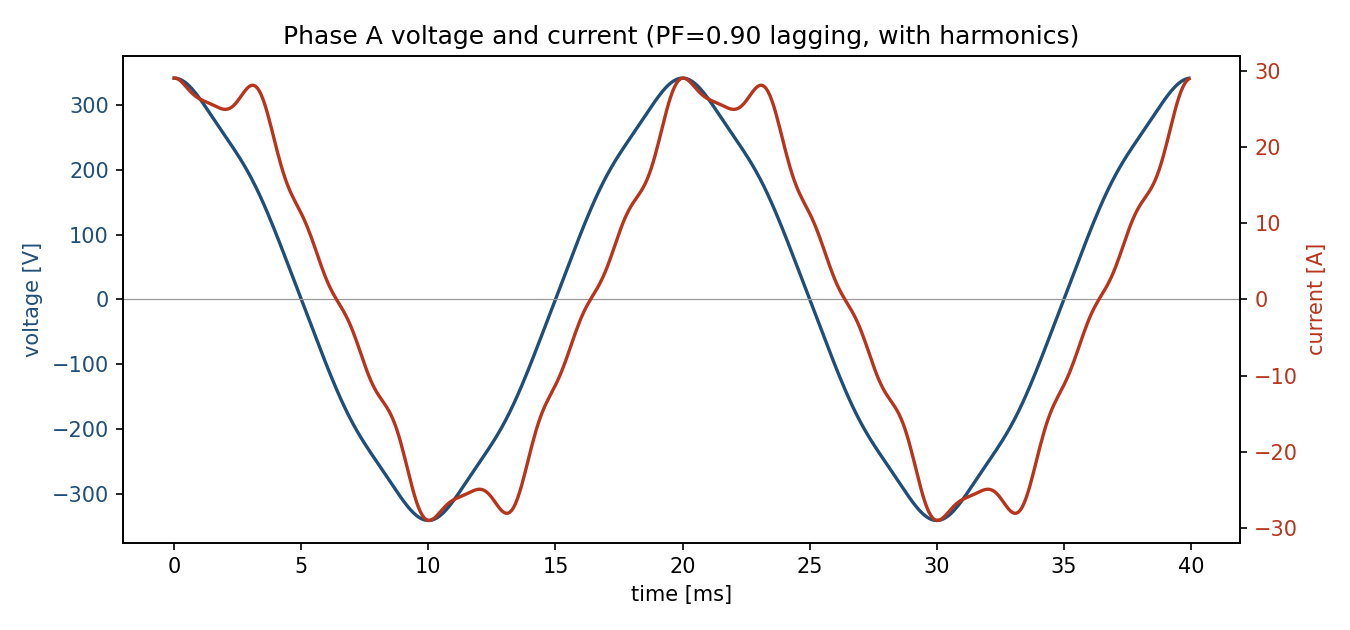
\includegraphics[width=0.9\textwidth]{waveforms.png}
\caption{Synthetic phase-A voltage and current (0.90 lagging, with harmonics).}
\label{fig:wave}
\end{figure}

\begin{figure}[h]
\centering
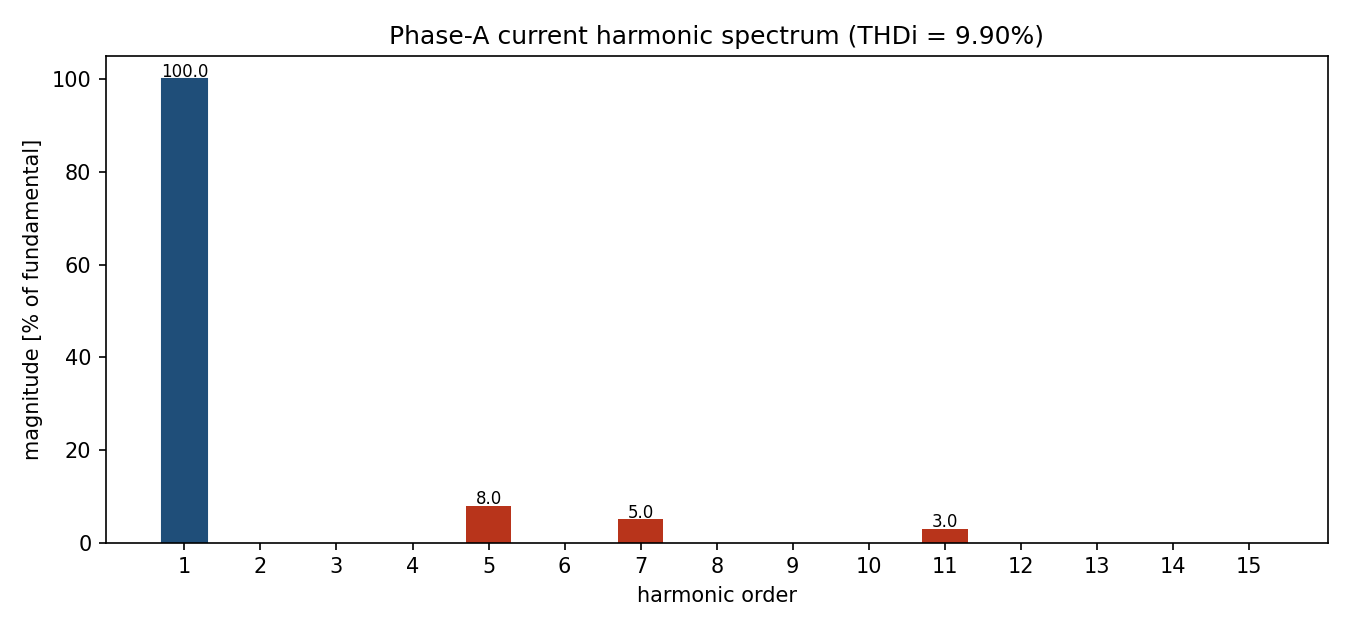
\includegraphics[width=0.9\textwidth]{spectrum.png}
\caption{Phase-A current harmonic spectrum; the 5th, 7th and 11th orders dominate the distortion.}
\label{fig:spec}
\end{figure}

\section{Results}
Table~\ref{tab:val} lists the firmware output against the numpy reference for phase A. All
quantities agree to at least five significant figures; the largest relative error is
$6.7\times10^{-5}$, on the THD values, and traces to the firmware using single precision while the
reference uses double. The measured THD equals the injected content exactly
($\mathrm{THD}_v=3.082\%$, $\mathrm{THD}_i=9.899\%$), confirming that the harmonic evaluation and
the summation are correct. Figure~\ref{fig:val} plots the per-metric relative error, all well
inside a 0.01\% band.

\begin{table}[h]
\centering
\caption{Firmware DSP versus independent numpy reference (phase A).}
\label{tab:val}
\begin{tabular}{lrrr}
\toprule
Quantity & Firmware (C) & Reference (numpy) & Rel.\ error \\
\midrule
$V_{rms}$ [V]   & 230.1092 & 230.1092 & $1.1\times10^{-7}$ \\
$I_{rms}$ [A]   & 20.0978  & 20.0978  & $1.9\times10^{-6}$ \\
$P$ [W]         & 4149.711 & 4149.712 & $1.3\times10^{-7}$ \\
$S$ [VA]        & 4624.680 & 4624.680 & $4.4\times10^{-8}$ \\
$PF$            & 0.89730  & 0.89730  & $3.4\times10^{-6}$ \\
$\mathrm{THD}_v$ & 0.03082 & 0.03082  & $6.7\times10^{-5}$ \\
$\mathrm{THD}_i$ & 0.09899 & 0.09899  & $5.0\times10^{-5}$ \\
\bottomrule
\end{tabular}
\end{table}

\begin{figure}[h]
\centering
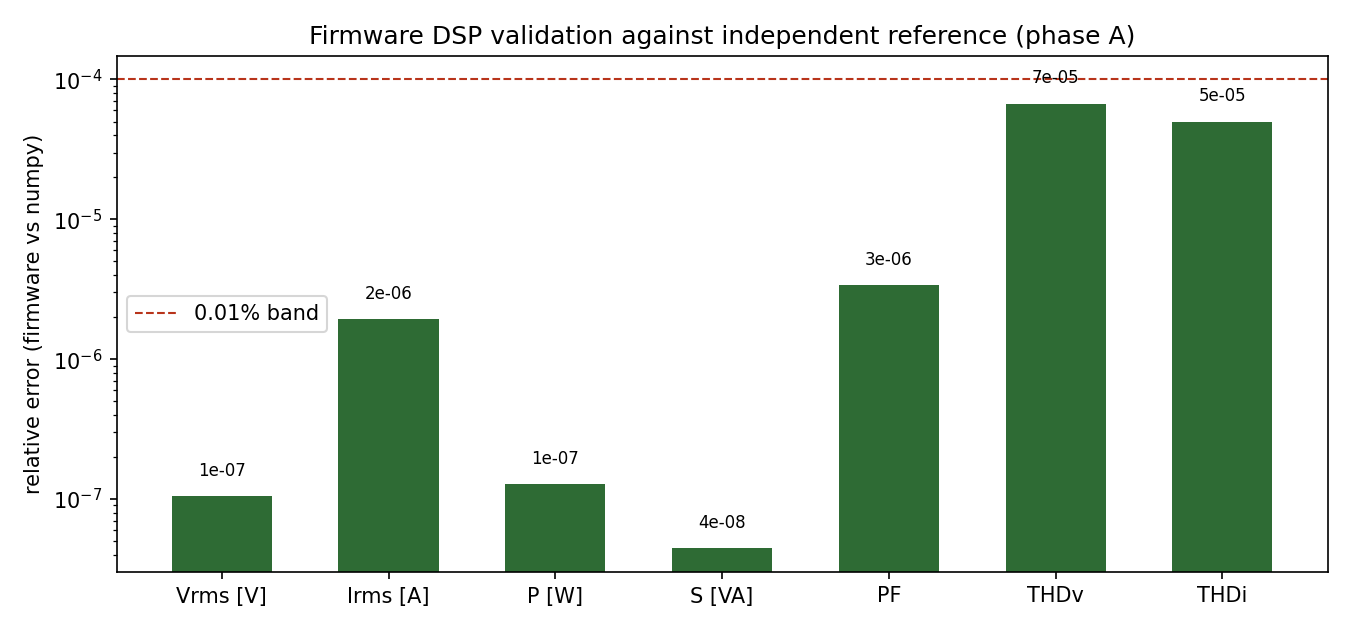
\includegraphics[width=0.9\textwidth]{validation.png}
\caption{Per-metric relative error of the firmware core against the reference (log scale).}
\label{fig:val}
\end{figure}

The true power factor comes out as 0.897, below the 0.90 fundamental displacement factor set in
the test; the 9.9\% current distortion accounts for the difference, as expected from the true-RMS
definition. The three-phase active power is 12.45~kW.

\section{Conclusion}
The measurement core of a three-phase energy analyzer was implemented for the ESP32 and verified
by compiling the identical C source on a host and comparing it against an independent reference
over synthetic waveforms with known harmonics. Agreement to $6.7\times10^{-5}$ and the exact
recovery of the injected THD give confidence that the algorithm is correct ahead of hardware
bring-up. The remaining work---ADC timing, front-end calibration and field verification against a
reference meter---is hardware-specific and left for commissioning.

\begin{thebibliography}{9}
\bibitem[Goertzel (1958)]{goertzel1958}
Goertzel, G. (1958). An algorithm for the evaluation of finite trigonometric series.
\textit{The American Mathematical Monthly, 65}(1), 34--35. https://doi.org/10.2307/2310304

\bibitem[IEC (2002)]{iec4007}
International Electrotechnical Commission. (2002). \textit{IEC 61000-4-7 Electromagnetic
compatibility (EMC) -- Part 4-7: Testing and measurement techniques -- General guide on harmonics
and interharmonics measurements and instrumentation}. IEC.

\bibitem[IEC (2015)]{iec4030}
International Electrotechnical Commission. (2015). \textit{IEC 61000-4-30 Electromagnetic
compatibility (EMC) -- Part 4-30: Testing and measurement techniques -- Power quality measurement
methods}. IEC.

\bibitem[IEEE (2010)]{ieee1459}
Institute of Electrical and Electronics Engineers. (2010). \textit{IEEE Std 1459-2010 -- IEEE
standard definitions for the measurement of electric power quantities under sinusoidal,
nonsinusoidal, balanced, or unbalanced conditions}. IEEE. https://doi.org/10.1109/IEEESTD.2010.5439063
\end{thebibliography}

\end{document}
